\documentclass[a4paper]{article}
\usepackage{calc,amsmath,amssymb,amsfonts}
\usepackage[T2A,T1]{fontenc}
\usepackage[russian]{babel}
\usepackage{xcolor,longfbox,fancyhdr}
\usepackage[margin=1in,noheadfoot]{geometry}
\usepackage{array,supertabular,hhline,enumitem,hyperref}
\hypersetup{colorlinks=true,allcolors=blue,pdfauthor=Инкогнито Грешитель}
\usepackage[pdftex]{graphicx}
\makeatletter\newdimen\@tempdimd\makeatother
% Outline numbering
\setcounter{secnumdepth}{0}
\makeatletter
\newcommand\arraybslash{\let\\\@arraycr}
\makeatother
% Pages
\fancypagestyle{Standard}{\fancyhf{}
  \fancyhead[L]{}
  \fancyfoot[L]{}
  \renewcommand\headrulewidth{0pt}
  \renewcommand\footrulewidth{0pt}
  \renewcommand\thepage{\arabic{page}}
}
\pagestyle{Standard}
\setlength\tabcolsep{1mm}
\renewcommand\arraystretch{1.3}
\author{Инкогнито Грешитель}
\date{2024-10-04}
\begin{document}
\clearpage
\pagestyle{Standard}

\foreignlanguage{russian}{\textbf{2. Построение графика значений для заданной числовой последовательности.}}

\foreignlanguage{russian}{График данной последовательности имеет следующий вид:}


\lfbox[margin-right=0.1256in,margin-left=0.1256in,margin-top=0mm,margin-bottom=0mm,border-style=none,padding=0mm,vertical-align=top]{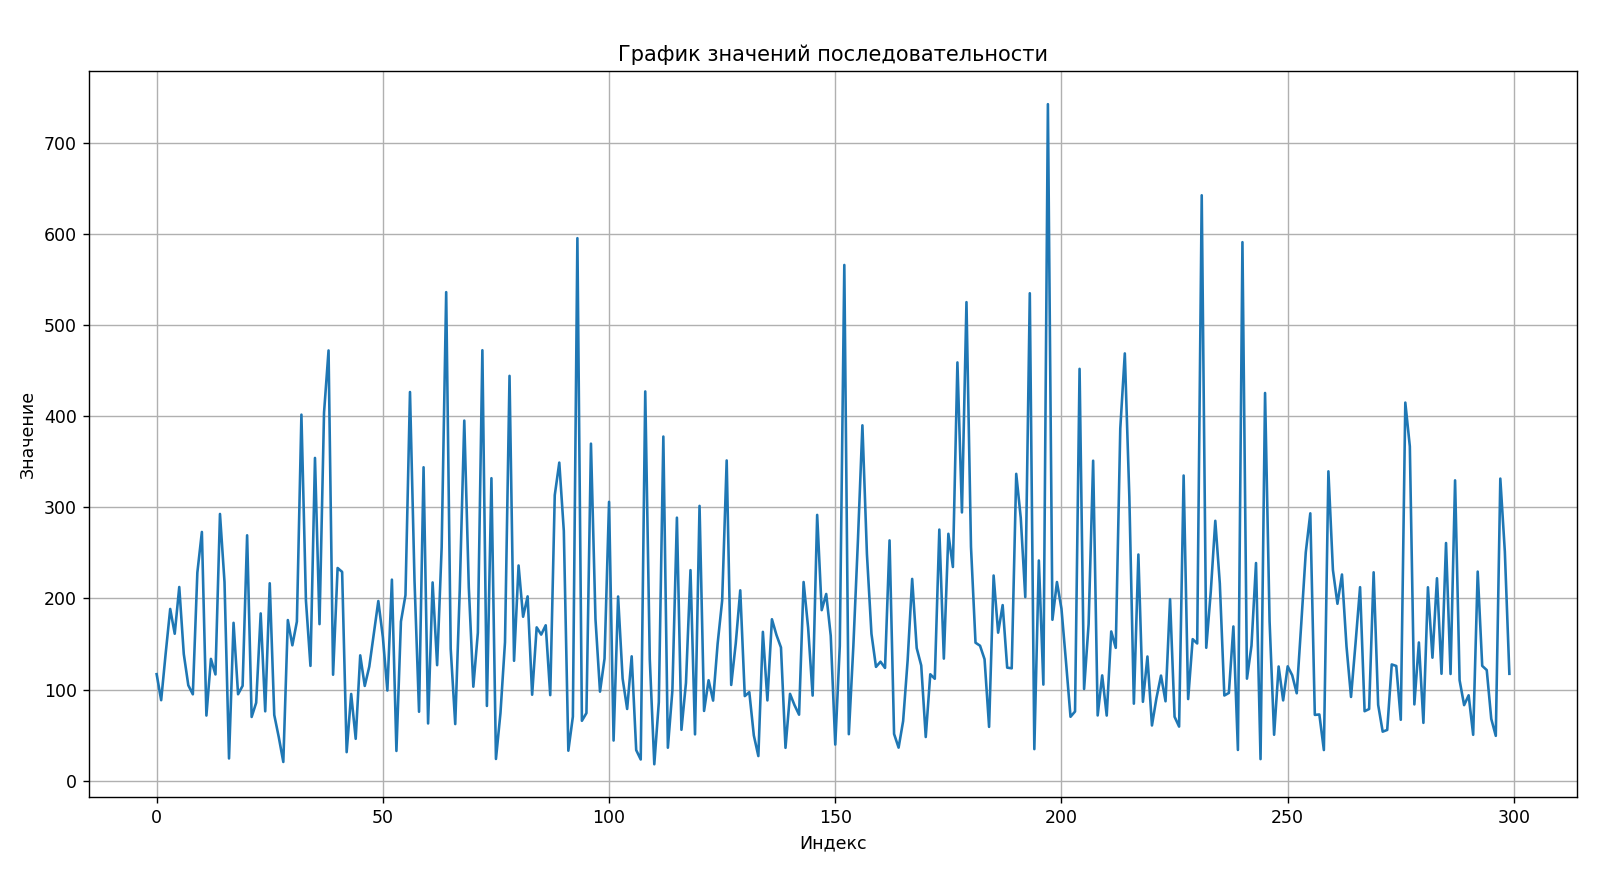
\includegraphics[width=7.0937in,height=4.0484in]{Posledovatelnost.png}}
\foreignlanguage{russian}{Очевидно, что данная последовательность не является возрастающей/невозрастающей, равно как и
не является убывающей/неубывающей. Можно было бы сказать, что последовательность отдалённо похожа на периодическую,
однако у неё отсутствует какой-либо повторяющийся за единицу времени паттерн.}\newline
\newline
\foreignlanguage{russian}{\textbf{3. Автокорреляционный анализ}}

\begin{flushleft}
\tablefirsthead{}
\tablehead{}
\tabletail{}
\tablelasttail{}
\begin{supertabular}{|m{0.81505984in}|m{0.5275598in}|m{0.5879598in}|m{0.47335985in}|m{0.5358598in}|m{0.5775598in}|m{0.5045598in}|m{0.5566598in}|m{0.5150598in}|m{0.5156598in}|m{0.49275985in}|}
\hline
\centering \foreignlanguage{russian}{\textbf{Сдвиг ЧП}} &
\centering \foreignlanguage{russian}{1} &
\centering \foreignlanguage{russian}{2} &
\centering \foreignlanguage{russian}{3} &
\centering \foreignlanguage{russian}{4} &
\centering \foreignlanguage{russian}{5} &
\centering \foreignlanguage{russian}{6} &
\centering \foreignlanguage{russian}{7} &
\centering \foreignlanguage{russian}{8} &
\centering \foreignlanguage{russian}{9} &
\centering\arraybslash \foreignlanguage{russian}{10}\\\hline
\centering \foreignlanguage{russian}{\textbf{К-т АК}}\foreignlanguage{russian}{ для задан.
}\foreignlanguage{russian}{\textbf{ЧП}} &
\centering \foreignlanguage{russian}{{}-0.0206} &
\centering \foreignlanguage{russian}{{}-0.0099} &
\centering \foreignlanguage{russian}{0.0579} &
\centering \foreignlanguage{russian}{0.068} &
\centering \foreignlanguage{russian}{{}-0.016} &
\centering \foreignlanguage{russian}{{}-0.0047} &
\centering \foreignlanguage{russian}{0.017} &
\centering \foreignlanguage{russian}{{}-0.0307} &
\centering \foreignlanguage{russian}{{}-0.0334} &
\centering\arraybslash \foreignlanguage{russian}{{}-0.026}\\\hline
\centering \foreignlanguage{russian}{\textbf{К-т АК}}\foreignlanguage{russian}{ для сгенерир.
}\foreignlanguage{russian}{\textbf{ЧП}} &
\centering \foreignlanguage{russian}{{}-0.0464} &
\centering \foreignlanguage{russian}{0.0167} &
\centering \foreignlanguage{russian}{0.0242} &
\centering \foreignlanguage{russian}{{}-0.035} &
\centering \foreignlanguage{russian}{0.0909} &
\centering \foreignlanguage{russian}{{}-0.056} &
\centering \foreignlanguage{russian}{{}-0.0495} &
\centering \foreignlanguage{russian}{{}-0.0452} &
\centering \foreignlanguage{russian}{{}-0.0632} &
\centering\arraybslash \foreignlanguage{russian}{{}-0.0089}\\\hline
\centering \foreignlanguage{russian}{\textbf{\%}} &
\centering \foreignlanguage{russian}{125.243} &
\centering \foreignlanguage{russian}{{}-268.687} &
\centering \foreignlanguage{russian}{{}-58.204} &
\centering \foreignlanguage{russian}{{}-151.471} &
\centering \foreignlanguage{russian}{{}-668.125} &
\centering \foreignlanguage{russian}{1091.49} &
\centering \foreignlanguage{russian}{{}-391.176} &
\centering \foreignlanguage{russian}{47.231} &
\centering \foreignlanguage{russian}{89.222} &
\centering\arraybslash \foreignlanguage{russian}{{}-65.769}\\\hline
\end{supertabular}
\end{flushleft}

\lfbox[margin-right=0.1256in,margin-left=0.1256in,margin-top=0mm,margin-bottom=0mm,border-style=none,padding=0mm,vertical-align=top]{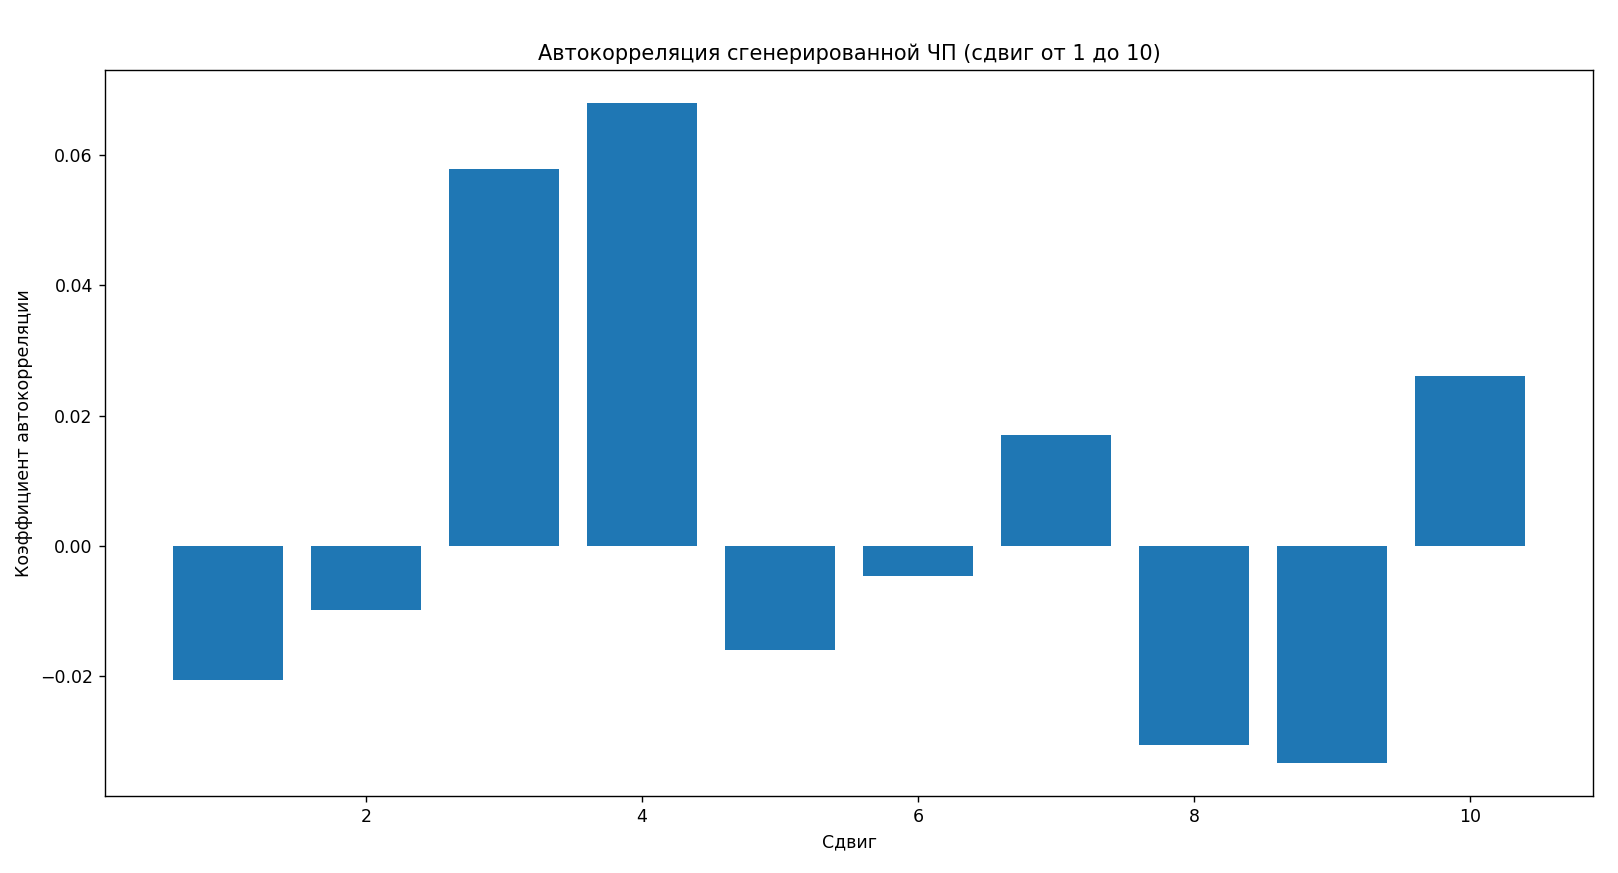
\includegraphics[width=6.2602in,height=3.3752in]{AutoCor1.png}}


Автокорреляция в сути своей показывает зависимость между текущими данными с предыдущими значениями для выявления
тенденций в последовательностях (т.е. чтобы по предыдущим значениям мы имели возможность предсказать
следующие).\newline
В качестве порогового значения, превышение которого говорит о том, что последовательность неслучайна, нами было выбрано
значение 0.2, и, как мы убедились во время проведения работы, ни для одного из сдвигов коэффициенты автокорреляции не
превышали даже 0.1, из чего мы можем предполагать, что заданная числовая последовательность является случайной.


\lfbox[margin-right=0.1256in,margin-left=0.1256in,margin-top=0mm,margin-bottom=0mm,border-style=none,padding=0mm,vertical-align=top]{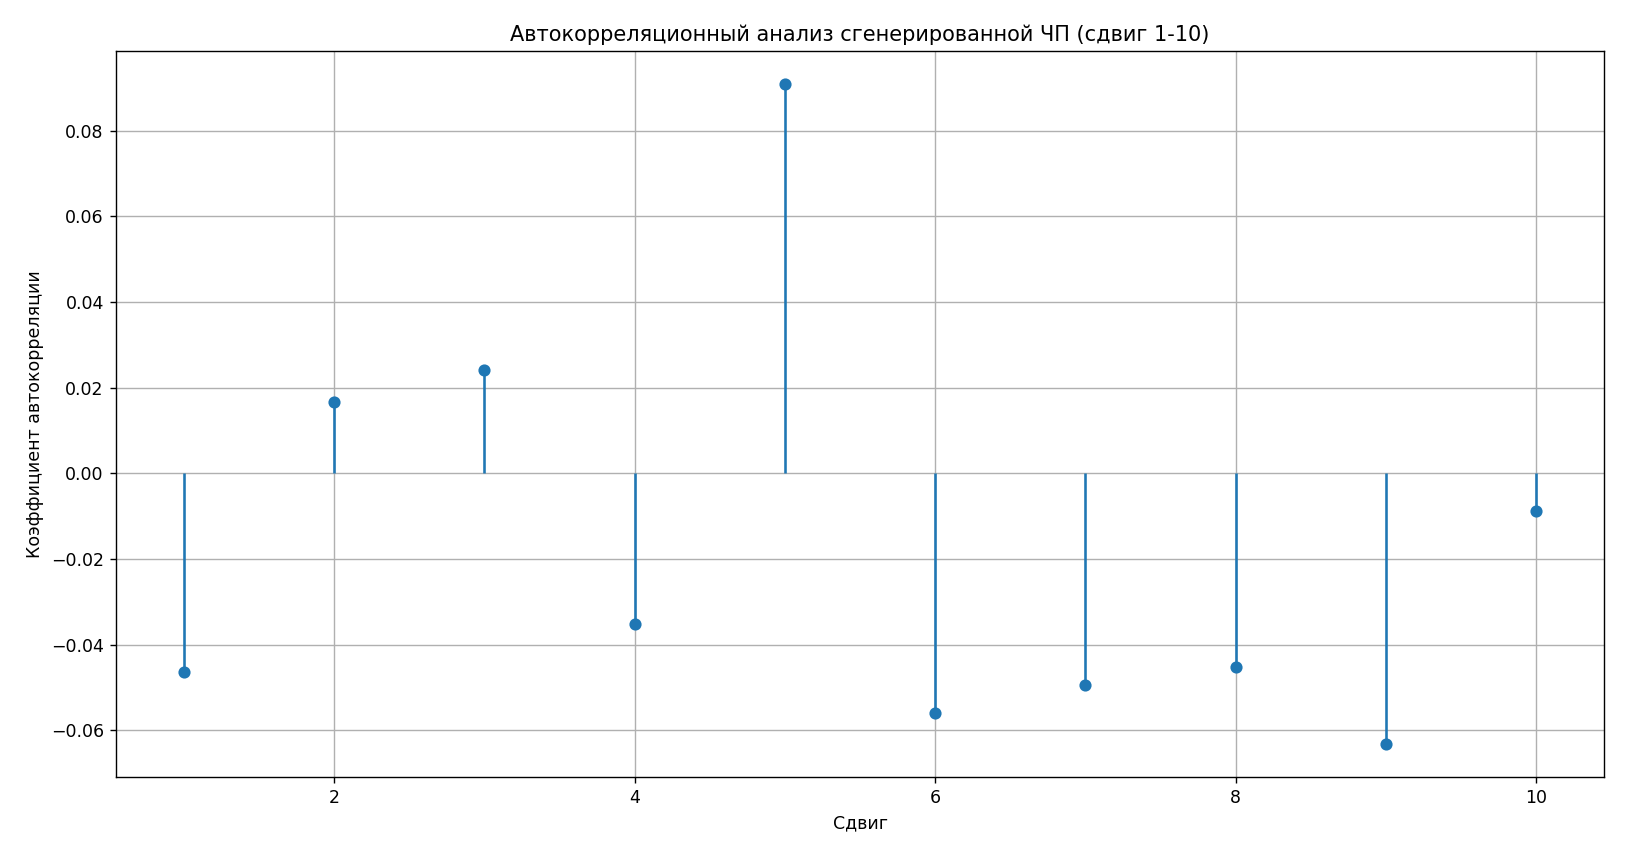
\includegraphics[width=5.8701in,height=3.048in]{AutoCor2.png}}


Автокорреляционный анализ сгенерированной числовой последовательности даёт нам аналогичные результаты: ни одно из
значений коэффициентов автокорреляции не превышало 0.1, не говоря уже о 0.2, из чего мы можем делать вывод, что
генерируемая нами последовательность не только случайна, но и приближена к заданной.
\end{document}
